\documentclass[11pt,a4paper]{article}

\usepackage[T1]{fontenc}
\usepackage[utf8]{inputenc}
\usepackage{mathptmx}
\usepackage{courier}
\usepackage[margin=2.5cm]{geometry}
\usepackage{amsmath}
\usepackage{booktabs}
\usepackage{graphicx}
\usepackage{xcolor}
\usepackage[numbers,sort&compress]{natbib}
\usepackage{xurl}
\usepackage[hidelinks]{hyperref}
\hypersetup{pdftitle={Routers and Cascades Miss a 15-Point Oracle Gap in Multi-Agent RAG},pdfauthor={Muzammal Hussain}}
\usepackage{caption}
\captionsetup{font=small,labelfont=bf}

\newcommand{\code}[1]{\texttt{#1}}
\setlength{\emergencystretch}{3em}

\title{\textbf{Routers and Cascades Miss a 15-Point Oracle Gap\\in Multi-Agent RAG}}
\author{Muzammal Hussain\\
\small Independent researcher, Glasgow, United Kingdom\\
\small \href{mailto:muzammal@masmatixinnovations.co.uk}{muzammal@masmatixinnovations.co.uk}\\
\small ORCID: \href{https://orcid.org/0009-0001-2570-5686}{0009-0001-2570-5686}}
\date{\small November 2026}

\begin{document}
\maketitle

\begin{abstract}
\noindent
A system with several retrieval-augmented agents of different cost can save compute by sending each question to the
cheapest agent that will answer it correctly. We measure how much of that saving is reachable in practice. Five agents
built from Qwen2.5 1.5B and 7B (no retrieval, one retrieval step, or iterative retrieval) answered 2,000 questions
from NQ-Open, SQuAD, HotpotQA and MuSiQue over one pooled corpus, with every answer scored and its compute measured.
On the 300 test questions an oracle that knows the cheapest correct agent reaches 61.0\% accuracy at 61\% of the
compute of the strongest agent, which alone reaches 45.7\%. We compare this ceiling with the fixed-agent mix, the
best accuracy reachable at each compute by sending a fixed share of questions to each agent. A gated neural router,
logistic regression and $k$-nearest neighbours over question embeddings all stayed within 1.5 points of that
mix (5 seeds for the neural router; exact McNemar $p \ge 0.33$ against the strongest agent), and the neural router
was not better than the two simple baselines. Answer-level cascades, which run the small agents first and escalate
when their answers disagree, refuse or look unreliable, did no better: the best matched the strongest agent's
accuracy (46.0\%) at 110\% of its compute, because 92\% of questions were escalated. Even a cascade that knew exactly
when the small retrieval agent was right would reach only 50.0\%. The remaining 11 points come from questions that
only the other agents answered, so the oracle's gain reflects agents that are right on different questions, which
neither the question nor the cheap answers revealed here. Data, code, all answers and costs are public.
\end{abstract}

\noindent\textbf{Keywords:} retrieval-augmented generation; LLM routing; model cascades; multi-agent systems; compute cost; negative result

\section{Introduction}

Retrieval-augmented question answering can be run in many ways: a small or large model, with or without retrieval,
with one retrieval step or several. The cheaper configurations answer many questions correctly, so a system that sent
each question to the cheapest configuration able to answer it would save compute without losing accuracy. This idea
underlies learned LLM routers~\cite{ong2024routellm}, cascades that call a stronger model only when a cheaper one
looks unreliable~\cite{chen2023frugalgpt}, and adaptive retrieval that chooses a strategy from the question's
complexity~\cite{jeong2024adaptiverag}.

How much is there to gain, and how much of it can a router actually recover? We built five agents of increasing cost,
ran every agent on every question, and recorded correctness and compute for each answer. This gives the oracle, the
best possible routing, and lets any policy be scored exactly, without running models again. We then asked two
questions. Can a router that sees only the question choose well enough to beat a fixed mix of agents at the same
compute? And can a cascade that also sees the answers of cheap agents do better?

Our contributions are:
\begin{itemize}
  \item a routing dataset of 2,000 questions from four public benchmarks, answered by five agents over one pooled
  corpus, with correctness and measured compute for all 10,000 answers;
  \item a fair comparison of a gated neural router with logistic regression, $k$-nearest neighbours and the
  fixed-agent mix, on the same compute range, with five seeds, bootstrap intervals and exact McNemar tests;
  \item answer-level cascades using agreement, refusal and retrieval signals, with the ceiling of the cascade design;
  \item a negative result with a mechanism: the oracle's 15-point gain comes mostly from questions that only an agent
  other than the small retrieval agent and the strongest agent answers, which neither question-only routers nor small-then-large cascades capture.
\end{itemize}

\section{Related work}

\paragraph{Routing between models.} RouteLLM~\cite{ong2024routellm} trains routers between a strong and a weak LLM
from preference data and reports large cost savings at near-strong quality. FrugalGPT~\cite{chen2023frugalgpt}
combines prompt adaptation, approximation and an LLM cascade in which a scorer decides whether to accept an answer or
call the next model. We study the same two ideas, question-level routing and answer-level cascades, with five agents
rather than two, and with the fixed-agent mix as the baseline that a router has to beat. Hybrid
LLM~\cite{ding2024hybrid} routes each query to a small or a large model from predicted difficulty, with a quality
level that can be tuned at test time. AutoMix~\cite{aggarwal2024automix} lets a small model check its own answer and
uses a POMDP-based router to decide whether to call a larger model, which is close to our answer-level cascades.
RouterBench~\cite{hu2024routerbench} provides a benchmark and dataset of model outputs for comparing routers on
cost and quality; we follow its practice of judging routers against non-learned baselines on a shared cost axis.

\paragraph{Adaptive retrieval.} Adaptive-RAG~\cite{jeong2024adaptiverag} trains a classifier that predicts question
complexity and chooses between no retrieval, single-step retrieval and iterative retrieval in the style of
IRCoT~\cite{trivedi2023ircot}. Our agents span the same three strategies and two model sizes, and we compare a
learned router with simple baselines on exactly measured compute.

\section{Method}

\paragraph{Agents.} All agents use instruction-tuned Qwen2.5 models~\cite{qwen2025qwen25} with greedy decoding and one
shared prompt format. \code{A\_direct\_small} (1.5B) and \code{B\_direct\_large} (7B) answer without retrieval.
\code{C\_rag\_small} (1.5B) and \code{D\_rag\_large} (7B) retrieve five passages once. \code{E\_iterative\_large}
(7B) alternates reasoning and retrieval for up to three steps (three passages per step, at most nine in total).
Retrieval is exact dense search with \code{multilingual-e5-base}~\cite{wang2024me5}. Compute per answer is estimated
as $2 \times \text{parameters} \times \text{tokens processed}$~\cite{kaplan2020scaling}, summed over all calls an
agent makes. Agents are ordered by mean compute, from A to E.

\paragraph{Questions.} We sampled 500 questions from the validation split of each of NQ-Open~\cite{lee2019latent,
kwiatkowski2019nq}, SQuAD v1.1~\cite{rajpurkar2016squad}, HotpotQA (distractor)~\cite{yang2018hotpotqa} and
MuSiQue-Ans~\cite{trivedi2022musique}. All paragraphs are pooled into one corpus, so retrieval faces distractors from
other questions and datasets. Splits are 70/15/15 (1,400/300/300 questions), stratified by dataset. An answer is
correct if it matches a gold answer exactly, contains it, or reaches token F1 $\ge 0.6$ after SQuAD normalisation.

\paragraph{Oracle and fixed-agent mix.} The oracle label of a question is the cheapest correct agent, or the
strongest agent if none is correct. Sending a random share of questions to each of two agents reaches any point on
the segment between them, so the upper concave hull of the five agents in (compute, accuracy) is reachable without a
router. We call it the \emph{fixed-agent mix}; a policy is useful only where it is above it at the same compute.

\paragraph{Question-only routers.} All routers read the 768-dimensional question embedding. The neural router is an
MLP with a sigmoid feature gate (hidden size 384, LayerNorm, GELU, dropout 0.1), trained with AdamW and early
stopping on validation loss, with five seeds. It is trained either on the oracle label (cross-entropy; the top agent
is used unless its probability is below $\tau$, then the strongest) or on per-agent correctness (binary
cross-entropy; the cheapest agent with estimated $P(\text{correct}) \ge \tau$ is used, else the strongest). A
no-gate version is the ablation. Baselines are logistic regression and $k$-nearest neighbours ($k=15$) trained for
the same two targets.

\paragraph{Answer-level cascades.} A cascade runs one or two cheap agents, keeps \code{C\_rag\_small}'s answer if a
score reaches $\tau$, and otherwise runs an escalation agent and uses its answer; every agent that runs is paid for.
Signals, all available at inference time, are the token F1 and exact agreement between A's and C's answers, answer
lengths, a refusal flag (empty answers or phrases such as ``unknown'' or ``not mentioned''), and the cosine similarity
of C's best retrieved passage. We test an agreement rule (score = A--C token F1, escalate to E), logistic regression
on all signals (escalate to E or to D) and logistic regression on C's signals only (run C alone, escalate to E). A
\emph{perfect accept} cascade, which keeps C's answer exactly when it is correct, is the ceiling of this design.

\paragraph{Operating point and statistics.} For every learned policy, $\tau^*$ is chosen on the validation split as
the cheapest threshold within one point of the strongest agent's validation accuracy, then applied unchanged to the
test split. Whole accuracy--compute curves are compared by their mean accuracy over a compute range that every
compared curve covers. Accuracy intervals are 95\% bootstrap intervals over questions~\cite{efron1993bootstrap};
paired differences use exact McNemar tests~\cite{mcnemar1947}. For the correctness router we report the expected
calibration error (ECE, 10 bins)~\cite{guo2017calibration}. The runs used two Kaggle T4 GPUs for the agents; routers
and cascades are computed from the saved answers.

\section{Results}

\begin{table}[t]
\centering
\small
\caption{Single agents and the oracle on the 300 test questions. Compute is the mean per question; ``share'' is
relative to always using E.}
\label{tab:agents}
\begin{tabular}{lrrr}
\toprule
Policy & Accuracy (\%) [95\% CI] & TFLOPs & Share \\
\midrule
always A (1.5B, no retrieval) & 14.0 [10.3, 18.3] & 0.25 & 1.4\% \\
always B (7B, no retrieval) & 21.0 [16.7, 25.3] & 1.21 & 6.9\% \\
always C (1.5B, one retrieval) & 36.0 [30.7, 41.3] & 2.35 & 13.3\% \\
always D (7B, one retrieval) & 43.0 [37.3, 49.0] & 11.60 & 65.8\% \\
always E (7B, iterative) & 45.7 [40.0, 51.3] & 17.64 & 100\% \\
oracle (cheapest correct agent) & 61.0 [55.3, 66.3] & 10.83 & 61.4\% \\
\bottomrule
\end{tabular}
\end{table}

\paragraph{The ceiling.} Table~\ref{tab:agents} shows the agents and the oracle. B lies below the fixed-agent mix
(21.0\% against 24.1\% reachable at its compute), so mixes run through A, C, D and E. The oracle answers 61.0\% of
test questions at 61\% of E's compute, 15.3 points above E; on the other 39\% no agent is correct. Of the oracle's
extra 15.3 points, 4.3 come from questions that C answers and E does not, and 11.0 from questions that only A, B or D
answers.

\begin{figure}[t]
  \centering
  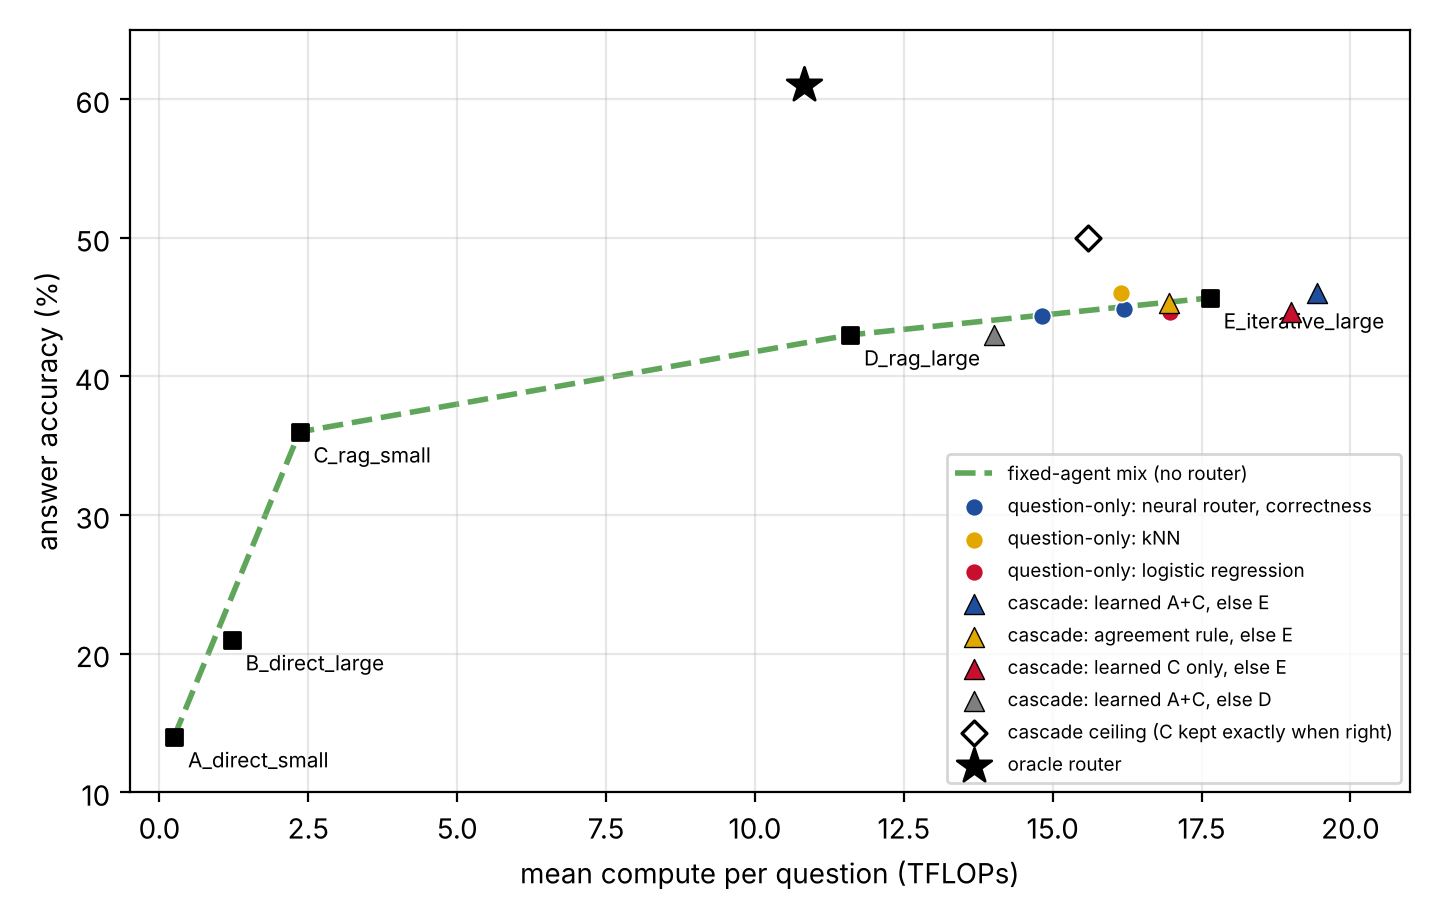
\includegraphics[width=0.92\linewidth]{figures/fig_policies.png}
  \caption{Accuracy against compute on the test split. Squares: single agents; dashed line: fixed-agent mix; circles:
  question-only routers at $\tau^*$ (both neural routers in blue); triangles: answer-level cascades at $\tau^*$;
  diamond: perfect-accept ceiling of the cascade design; star: oracle.}
  \label{fig:policies}
\end{figure}

\begin{table}[t]
\centering
\small
\caption{Learned policies on the test split. ``Gain'' is accuracy minus the fixed-agent mix at the same compute
(points). Neural routers: mean over five seeds. McNemar $p$ is against always E.}
\label{tab:policies}
\setlength{\tabcolsep}{4pt}
\begin{tabular}{lrrrr}
\toprule
Policy & Accuracy (\%) & Share of E & Gain & McNemar $p$ \\
\midrule
\multicolumn{5}{l}{\emph{Question-only routers}} \\
neural router, correctness (default $\tau=0.5$) & 45.0 $\pm$ 0.7 & 73.6\% & $+1.4$ & 0.56 \\
neural router, correctness @ $\tau^*$ & 44.9 $\pm$ 0.3 & 91.8\% & $-0.2$ & 0.55 \\
neural router, oracle label @ $\tau^*$ & 44.3 $\pm$ 0.4 & 84.0\% & $-0.1$ & 0.33 \\
$k$NN, oracle label @ $\tau^*$ & 46.0 & 91.5\% & $+1.0$ & -- \\
logistic regression, correctness @ $\tau^*$ & 44.7 & 96.3\% & $-0.7$ & 0.45 \\
\midrule
\multicolumn{5}{l}{\emph{Answer-level cascades (escalation rate in brackets)}} \\
agreement rule A+C, else E @ $\tau^*$ (77\%) & 45.3 & 96.2\% & $-0.0$ & 1.00 \\
learned A+C signals, else E @ $\tau^*$ (92\%) & 46.0 & 110.2\% & $+0.3$ & 1.00 \\
learned C signals only, else E @ $\tau^*$ (92\%) & 44.7 & 107.7\% & $-1.0$ & 0.25 \\
learned A+C signals, else D @ $\tau^*$ (98\%) & 43.0 & 79.4\% & $-1.1$ & 0.27 \\
perfect accept, else E (ceiling; 64\%) & 50.0 & 88.4\% & $+5.2$ & 0.0002 \\
\bottomrule
\end{tabular}
\end{table}

\paragraph{Question-only routers.} No question-only router was clearly better than the fixed-agent mix
(Table~\ref{tab:policies}, Figure~\ref{fig:policies}). On the compute range that all curves cover (15.6 to 17.6
TFLOPs per question), mean accuracy was 45.7\% for $k$NN, 45.6\% $\pm$ 0.2 for the correctness router, 45.2\% for
the fixed-agent mix, 45.0\% $\pm$ 0.1 for the oracle-label router and 44.7\% for logistic regression. The neural
router was not significantly different from the logistic-regression or $k$NN baselines at its operating points
(McNemar $p \ge 0.80$), nor from always using E ($p$ from 0.33 to 0.56). The neural routers and the baselines chose the oracle agent for 45 to
51\% of questions. The correctness router's probabilities were well calibrated (ECE 0.030 to 0.061 over seeds), so
the problem is not overconfidence: the question embedding carries little information about which agent will be
right. Removing the feature gate changed nothing (45.2\% $\pm$ 0.5 against 45.0\% $\pm$ 0.1 over the shared range;
44.4\% against 44.3\% at $\tau^*$).

\paragraph{Answer-level cascades.} Looking at cheap answers did not help either. At $\tau^*$ the best cascade
matched E's accuracy (46.0\% against 45.7\%) but used 110\% of E's compute: C is right on only 36\% of questions, so
92\% were escalated and the cost of running A and C was added to E's. Over the range 2.6 to 17.6 TFLOPs, mean accuracy
was 36.4 to 39.9\% for the four cascades against 41.5\% for the fixed-agent mix and 41.8\% for the question-only
logistic regression; no cascade curve rose more than 0.7 points above the mix anywhere. At the default threshold of
0.5 the learned A+C cascade was worse than E (42.3\% against 45.7\%, McNemar $p=0.041$). By dataset, the best cascade
escalated 80\% (HotpotQA) to 100\% (NQ-Open) of questions and used 101 to 118\% of E's compute; its accuracy equalled
E's on SQuAD (80.0\%), MuSiQue (22.7\%) and NQ-Open (17.3\%) and was 1.3 points higher on HotpotQA (64.0\% against
62.7\%).

\paragraph{The ceiling of a cascade.} Even with perfect knowledge of when C is right, a C-then-E cascade reaches
50.0\%, at 88\% of E's compute. It recovers the 4.3 points from questions that C answers and E does not, but not the
11.0 points from questions that only A, B or D answers, because it never asks those agents.

\section{Discussion}

\paragraph{The oracle overstates what routing can recover.} An oracle over five agents looks like a 15-point,
40\%-cheaper opportunity, but most of it comes from complementarity: different agents are right on different
questions, often not in order of cost. A router that sees only the question would need to predict which of five
agents succeeds on each question; here the embedding did not support that prediction better than a nearest-neighbour
lookup, and no learned router beat sending a fixed share of questions to each agent.

\paragraph{Cascades pay twice when the first step is weak.} A cascade saves compute only if the cheap agent is right
often enough and the signal for accepting its answer is reliable. With the small retrieval agent right on 36\% of
questions, most questions went to E anyway and the cheap step became overhead. Agreement, refusal and retrieval
signals did not separate C's correct answers well enough to change this.

\paragraph{Baselines that a router must beat.} Our neural router looks reasonable in isolation: it is well calibrated
and saves about a quarter of E's compute at 0.7 points below E's accuracy. Compared with the fixed-agent mix and with
$k$NN and logistic regression on the same features and compute range, it adds nothing. Routing studies should report
the fixed-agent mix and simple baselines on a shared compute range, not only savings against the strongest model.

\section{Limitations}

The agents come from one model family at two sizes, and other agent sets may be more or less complementary. Each
dataset contributed 500 questions, and the test split has 75 per dataset, so per-dataset results are uncertain; the
oracle and all policies were scored once with greedy decoding. Compute is estimated from parameters and tokens, not
measured as time or energy, and it counts only model inference: the cost of retrieval (embedding, index search and
re-ranking) is not included, which slightly favours agents that retrieve more often. Correctness uses a lenient rule (containment or F1 $\ge 0.6$), which may credit some
partly wrong answers. Cascade signals are simple; signals such as token probabilities, self-consistency over samples
or an LLM judge were not tested, and every cascade kept only the small retrieval agent's answer, so cascades that
choose among several agents' answers remain open. We did not test code-mixed questions.

\section{Conclusion}

Over 2,000 questions and five retrieval-augmented agents, perfect routing would add 15 points of accuracy at 61\% of
the strongest agent's compute. Neither a gated neural router, nor simple classifiers on the question, nor cascades
that check cheap agents' answers recovered any of this gain over a fixed mix of agents. The gain lies in agents that
are right on different questions, so progress needs signals that predict which agent will succeed, not only whether
a cheap answer can be trusted.

\section*{Code and data availability}

Code, the three Kaggle notebooks (oracle dataset, router training, answer-level cascades), the saved test-split
results and the figure script are at \url{https://github.com/MHKhan50/agentic-rag-router} and archived on
Zenodo (\href{https://doi.org/10.5281/zenodo.24339546}{doi:10.5281/zenodo.24339546}). The questions come from
public datasets under their own licences (NQ-Open and HotpotQA CC BY-SA, SQuAD CC BY-SA 4.0, MuSiQue CC BY 4.0);
derived data are released under CC BY-SA 4.0 and code under Apache 2.0.

\bibliographystyle{unsrtnat}
\bibliography{references}

\end{document}
